\section{Linear Models for the Quantile Autoregression}
\label{sec:linear-models}

Given a time series $\{y_t\}$, we investigate how to select which lags will be included in the Quantile Autoregression. We won't be choosing the full model because this normally leads to a bigger variance in our estimators, which is often linked with bad performance in forecasting applications. So our strategy will be to use some sort of regularization method in order to improve performance.
We investigate two ways of accomplishing this goal.
The first of them consists of selecting the best subset of variables through Mixed Integer Programming, given that $K$ variables are included in the model. Using MIP to select the best subset of variables is investigated in \cite{bertsimas2015best}. The second way is including a $\ell_1$ penalty on the linear quantile regression, as in \cite{kim2009ell_1}, and let the model select which and how many variables will have nonzero coefficients. 
Both of them will be built over the standard Quantile Linear Regression model. In the end of the section, we discuss a information criteria to be used for quantile regression and verify how close are the solutions in the eyes of this criteria.

When we choose $q(x_t)$ to be a linear function, as on equation \ref{eq:linear-model} (that we reproduce below for convenience):
\begin{equation}
\min_{f}\sum_{t=1}^{n}\alpha|y_{t}-q(x_t)|^{+}+(1-\alpha)|y_{t}-q(x_t)|^{-},
\end{equation}
we can substitute it on problem \ref{eq:qar-general}, getting the following LP problem:
\begin{equation}
\begin{aligned}\min_{\beta_0,\beta,\varepsilon_{t}^{+},\varepsilon_{t}^{-}} & \sum_{t=1}^{n}\left(\alpha\varepsilon_{t}^{+}+(1-\alpha)\varepsilon_{t}^{-}\right)\\
\mbox{s.t. } & \varepsilon_{t}^{+}-\varepsilon_{t}^{-}=y_{t} - \beta_0 - \beta^T x_{t},\qquad\forall t\in\{1,\dots,n\},\\
& \varepsilon_t^+,\varepsilon_t^- \geq 0, \qquad \forall t \in \{1,\dots,n\}.
\end{aligned}
\label{eq:qar-lp}
\end{equation}

In this work, we didn't explore the addition of terms other than the terms $y_t$ past lags. For example, we could include functions of $y_{t-p}$, such as $log(y_{t-p})$ or $exp(y_{t-p})$. We leave such inclusion for further works. 

\subsection{Best subset selection with Mixed Integer Programming}
\label{sec:best-subset-mip}

In this part, we investigate the usage of Mixed Integer Programming to select which variables are included in the model, up to a limit of inclusions imposed \textit{a priori}. The optimization problem is described below:
\begin{eqnarray}
\min_{\beta_{0},\beta, z,\varepsilon_{t}^{+},\varepsilon_{t}^{-}} &  \sum_{t=1}^{n}\left(\alpha\varepsilon_{t}^{+}+(1-\alpha)\varepsilon_{t}^{-}\right) \\
\mbox{s.t } & \varepsilon_{t}^{+}-\varepsilon_{t}^{-}=y_{t}-\beta_{0}-\sum_{p=1}^{P}\beta_{p}x_{t,p},& \qquad\forall t\in\{1,\dots,n\}, \label{linear1}\\
 & \varepsilon_{t}^{+},\varepsilon_{t}^{-}\geq0,&\qquad\forall t \in \{1,\dots,n\}, \label{linear2}\\
 & - M_U z_p \leq \beta_p \leq M_U z_p,&\qquad\forall p\in\{1,\dots,P\}, \label{linear3}\\
 & \sum_{p=1}^P z_p \leq K, \label{linear4}\\
 & z_p \in \{0,1\},&\qquad\forall p\in\{1,\dots,P\}. \label{eq:linear5}
\end{eqnarray}
The objective function and constraints (\ref{linear2}) and (\ref{linear3}) are those from the standard linear quantile regression. The other constraints implement the process of regularization, forcing a maximum of $K$ variables to be included. By (\ref{linear3}), variable $z_p$ is a binary that assumes 1 when the coefficient $\beta_p$ is included. $M_U$ is chosen in order to guarantee that $M_U \geq \|\hat{\beta}\|_{\infty}$. The solution given by $\beta_0$ and $\beta$ will be the best linear quantile regression with $K$ nonzero coefficients. 

We ran this optimization for each value of $K \in \{1, \dots, 12\}$ and quantiles $\alpha \in \{0.05, 0.1, 0.5, 0.9, 0.95\}$. We could see that for all quantiles the 12\textsuperscript{th} lag was the one included when $K=1$. When $K=2$, the 1\textsuperscript{st} lag was always included, sometimes with $\beta_{12}$, some others with $\beta_4$ and once with $\beta_{11}$. These 4 lags that were present until now are the only ones selected when $K=3$. For $K=4$, those same four lags were selected for three quantiles (0.05, 0.1 and 0.5), but for the others (0.9 and 0.95) we have $\beta_6$, $\beta_7$ and $\beta_9$ also as selected. From now on, the inclusion of more lags represent a lower increase in the fit of the quantile regression. The estimated coefficient values for all $K$'s are available in the appendices section. Figure \ref{fig:icaraizinho-crossing-200} shows a linear estimator for the quantiles $(0.05, 0.1, 0.25, 0.5, 0.75, 0.9, 0.95)$.

\begin{figure}
\centering
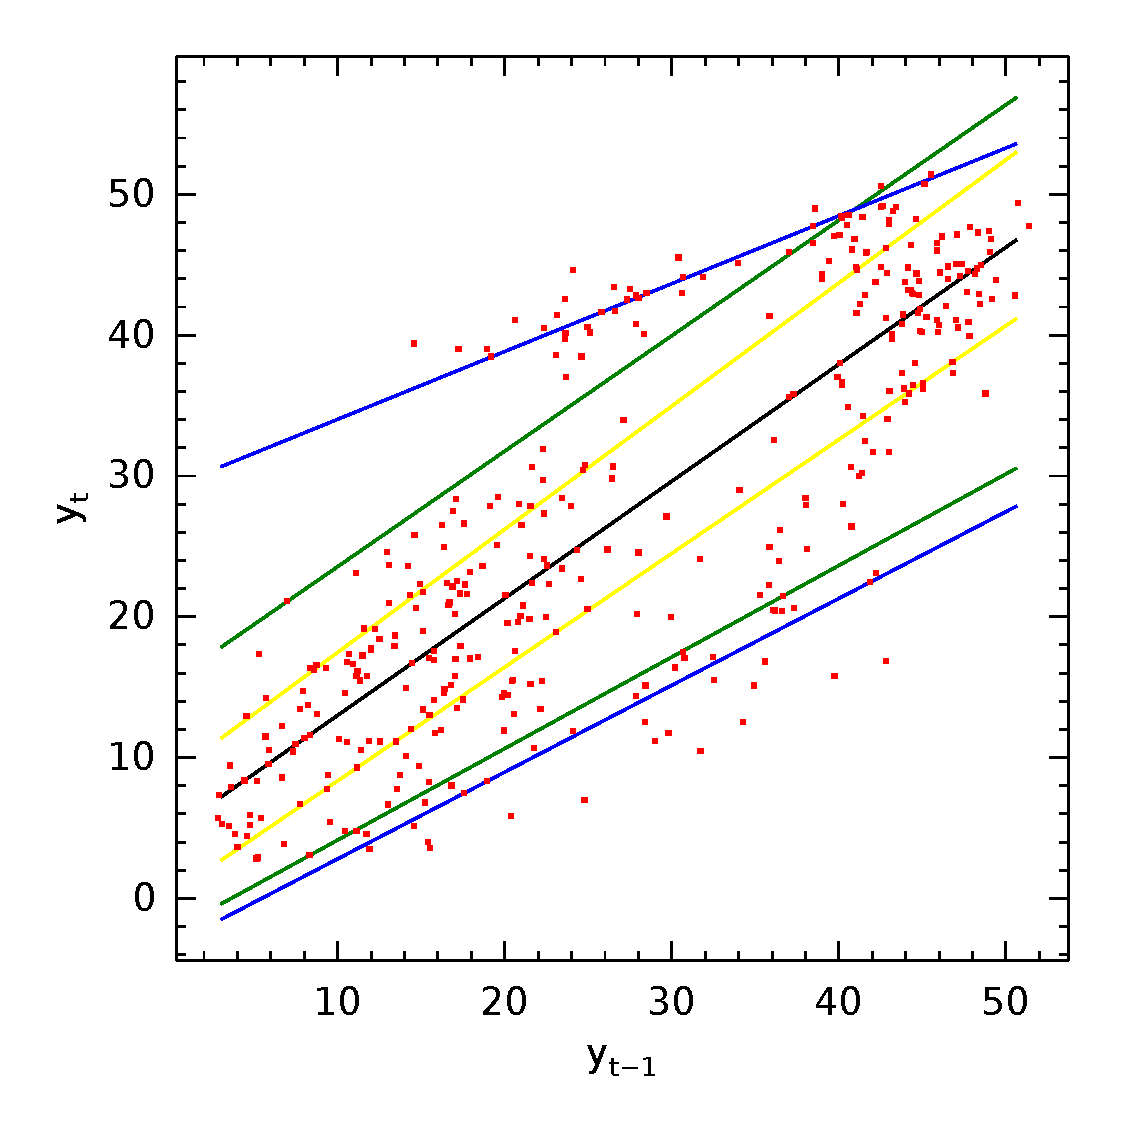
\includegraphics[width=0.7\linewidth]{Figuras/npqar/icaraizinho-crossing-200}
\caption{Linear Quantile Regression when only $y_{t-1}$ is used as explanatory variable}
\label{fig:icaraizinho-crossing-200}
\end{figure}


\subsection{Best subset selection with a $\ell_1$ penalty}
\label{sec:best-subset-ell1}

Another way of doing regularization is including the $\ell_1$-norm of the coefficients on the objective function. The advantage of this method is that coefficients are shrunk towards zero, and only some of them will have nonzero coefficients. By lowering the penalty we impose on the $\ell_1$-norm, more variables are being added to the model. 
This is the same strategy of the LASSO, and its usage for the quantile regression is discussed in \cite{li2012l1}.
The proposed optimization problem to be solved is:

\begin{equation}
\min_{\beta_{0},\beta}\sum_{t=1}^{n}\alpha|y_{t}-q(x_t)|^{+}+(1-\alpha)|y_{t}-q(x_t)|^{-}+\lambda\|\beta\|_{1}
\label{eq:l1-qar-optim}
\end{equation}
\[
q(x_t)=\beta_{0}-\sum_{p=1}^{P}\beta_{p}x_{t,p},
\]
where the regressors $x_{t,p}$ used are its lags. In order to represent the above problem to be solved with linear programming solver, we restructure the problem as below:
\begin{eqnarray}
\beta_\lambda^{*LASSO} = \argmin_{\beta_{0},\beta,\varepsilon_{t}^{+},\varepsilon_{t}^{-}} & \sum_{i=1}^{n}\left(\alpha\varepsilon_{t}^{+}+(1-\alpha)\varepsilon_{t}^{-}\right)+\lambda\sum_{p=1}^{P}\mbox{\ensuremath{\xi}}_{p} \label{eq:obj-lasso} \\
\mbox{s.t. } & \varepsilon_{t}^{+}-\varepsilon_{t}^{-}=y_{t}-\beta_{0}-\sum_{p=1}^{P}\beta_{p}x_{t,p},\qquad\forall t\in\{1,\dots,n\},\\
 & \varepsilon_{t}^{+},\varepsilon_{t}^{-}\geq0,\qquad\forall t \in \{1,\dots,n\},\\
 & \xi_{p}\geq\beta_{p},\qquad\forall p\in\{1,\dots,P\}, \label{l1-qar-3}\\
 & \xi_{p}\geq-\beta_{p},\qquad\forall p\in\{1,\dots,P\}, \label{l1-qar-4}
\end{eqnarray}
Once again, this model is built upon the standard linear programming model for the quantile regression (equation \ref{eq:qar-lp}). 
On the above formulation, the $\ell_1$ norm of equation (\ref{eq:l1-qar-optim}) is substituted by the sum of $\xi_p$, which represents the absolute value of $\beta_p$. The link between variables $\xi_p$ and $\beta_p$ is made by constraints (\ref{l1-qar-3}) and (\ref{l1-qar-4}). Note that the linear coefficient $\beta_0$ is not included in the penalization, as the sum of penalties on the objective function \ref{eq:obj-lasso}.

For such estimation to produce good results, however, each variable must have the same relative weight in comparison with one another. So, before solving the optimization problem, we normalize all variables to have mean $\mu = 0$ and variance $\sigma^2 = 1$. For the vector of observations for each covariate (that in our problem represents is a vector of observations of lags $y_{t-p}$), we apply the transformation $\tilde{y}_{t-p,i} = (y_{t-p,i} - \bar{y}_{t-p}) / \sigma_{t-p}$, where $\bar{y}_{t-p}$ is the $p$-lag mean and $\sigma_{t-p}$ the $p$-lag standard deviation. We use the $\tilde{y}_{t-p,i}$ series to estimate the coefficients. Once done that, we multiply each coefficient for its standard deviation to get the correct coefficient: $\beta_i = \tilde{\beta}_i \dot \sigma_{t-p}$.

For low values of $\lambda$, the penalty is small and thus we have a model where all coefficients have a nonzero value. On the other hand, while $\lambda$ is increased the coefficients shrink towards zero; in the limit we have a constant model. For instance, we don't penalize the linear coefficient $\beta_0$. For the same quantiles values $\alpha$ we experimented on section \ref{sec:best-subset-mip} ($\alpha \in \{0.05, 0.1, 0.5, 0.9, 0.95\}$). 


\begin{figure}
  \centering
  \begin{minipage}[t]{0.4\linewidth}
    \centering
    \begin{minipage}[t]{\linewidth}
      \centering     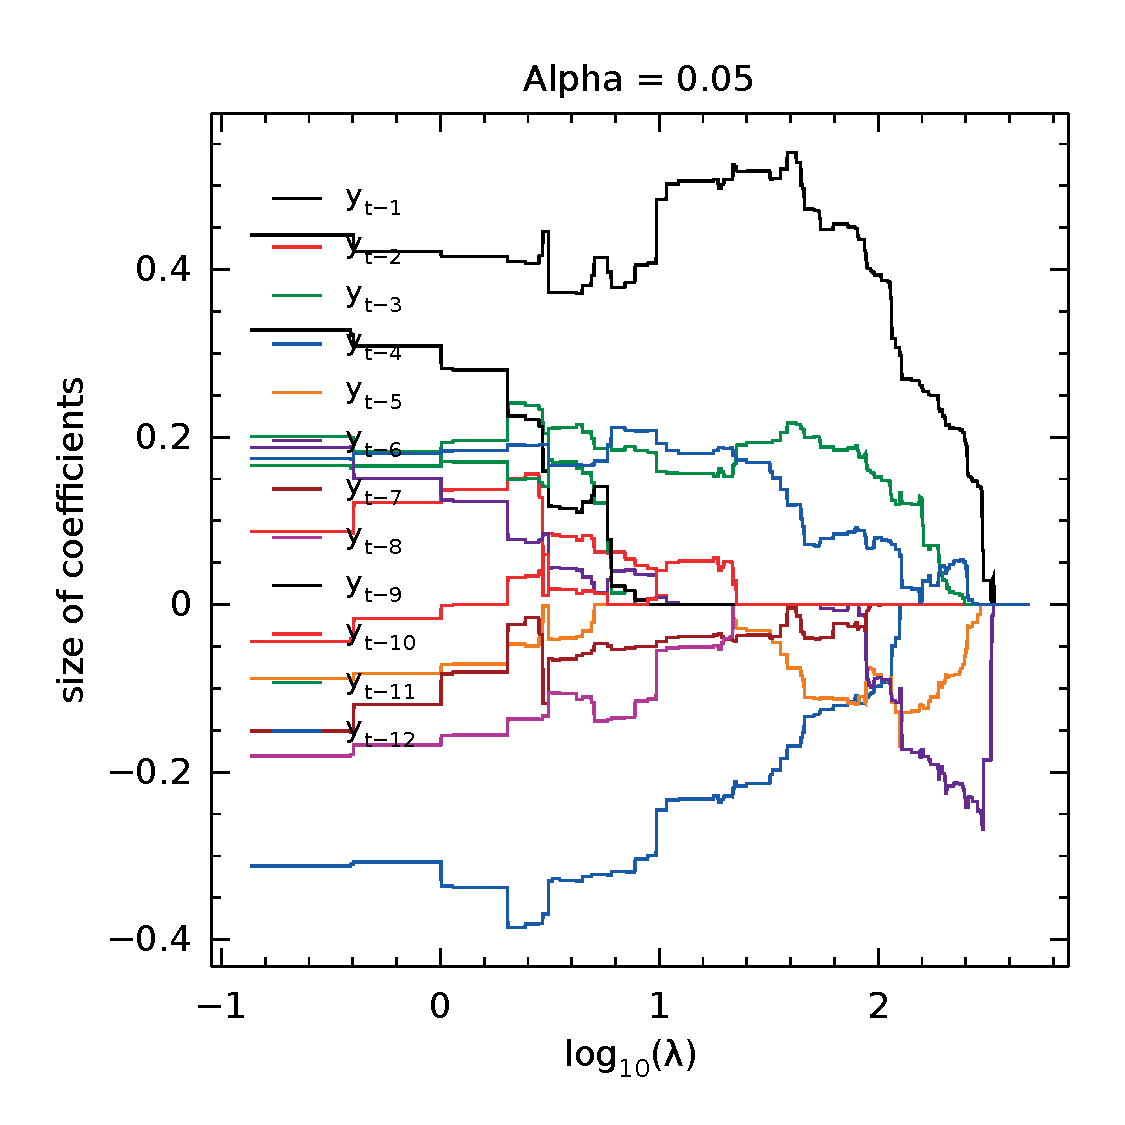
\includegraphics[width=\textwidth]{Figuras/selecao-lasso/par-sellasso-005.pdf}
    \end{minipage}
    \begin{minipage}[b]{\linewidth}
      \centering     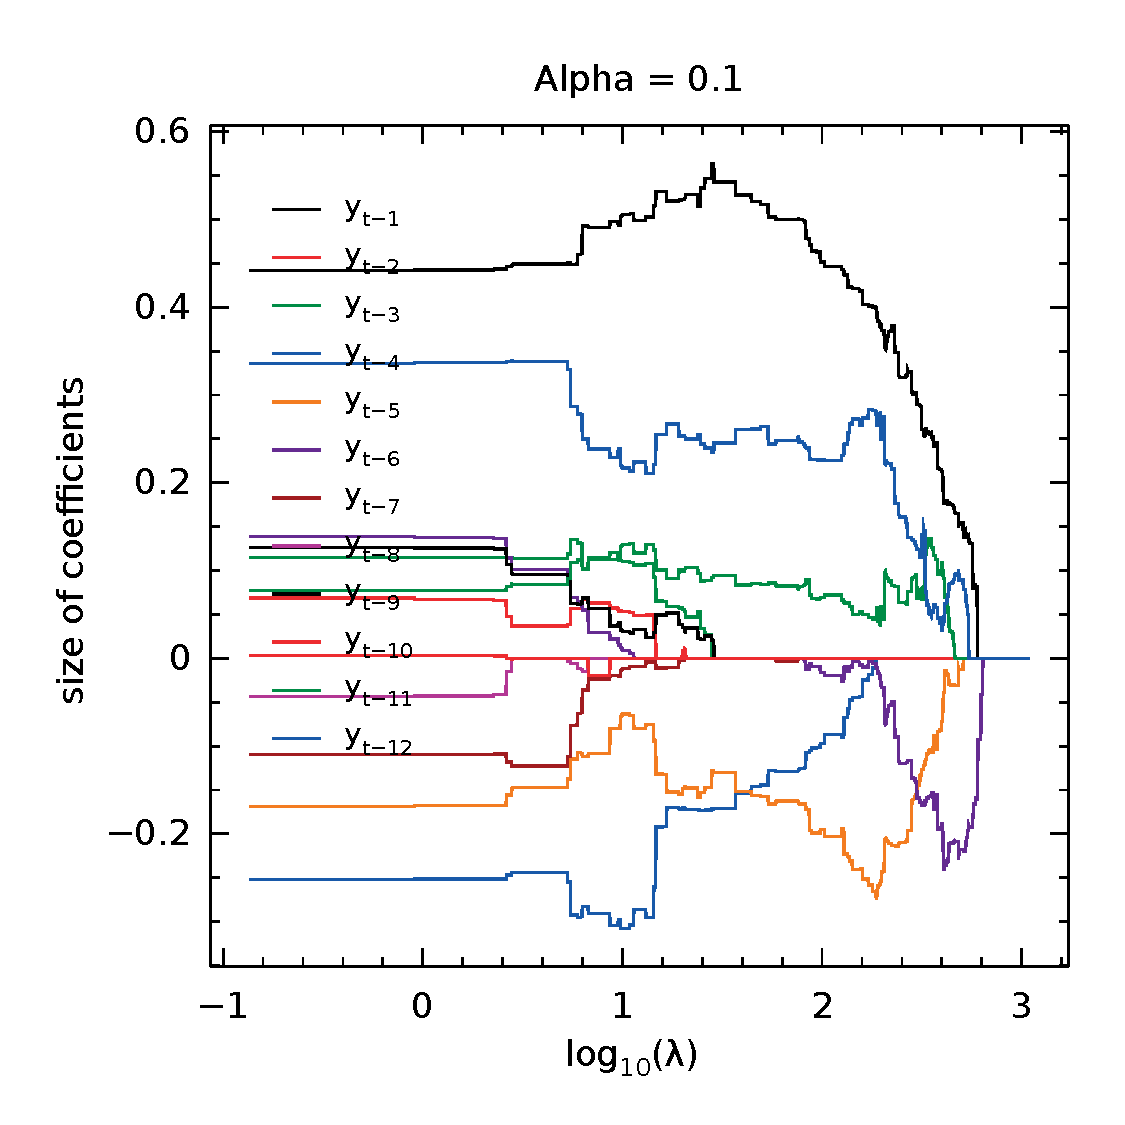
\includegraphics[width=\textwidth]{Figuras/selecao-lasso/par-sellasso-01.pdf}
    \end{minipage}
     \begin{minipage}[b]{\linewidth}
      \centering     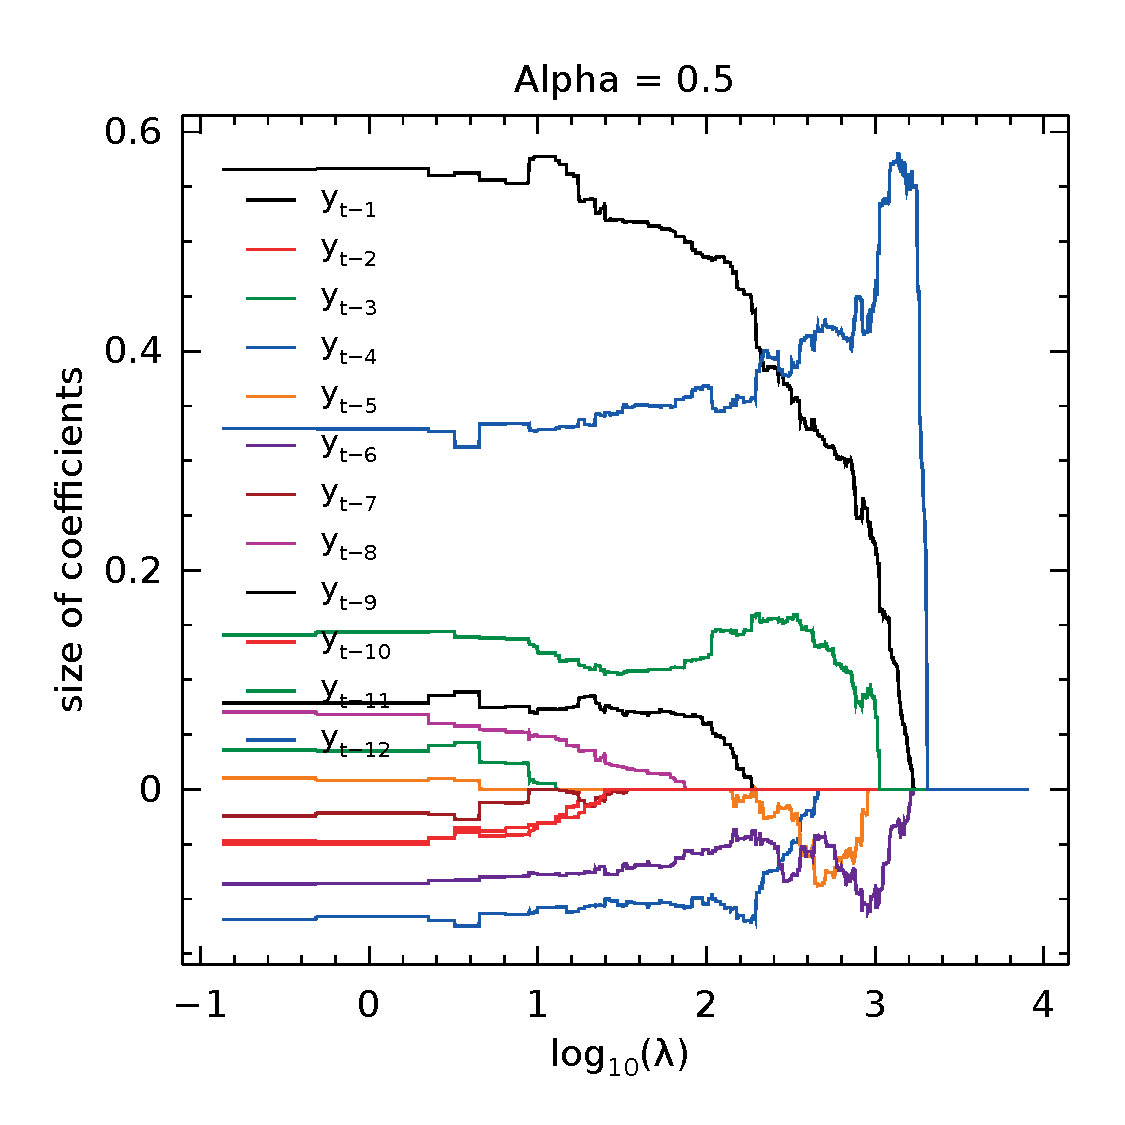
\includegraphics[width=\textwidth]{Figuras/selecao-lasso/par-sellasso-05.pdf}
     \end{minipage}
  \end{minipage}
  \begin{minipage}[t]{0.4\linewidth}
    \centering
    \begin{minipage}[b]{\linewidth}
      \centering     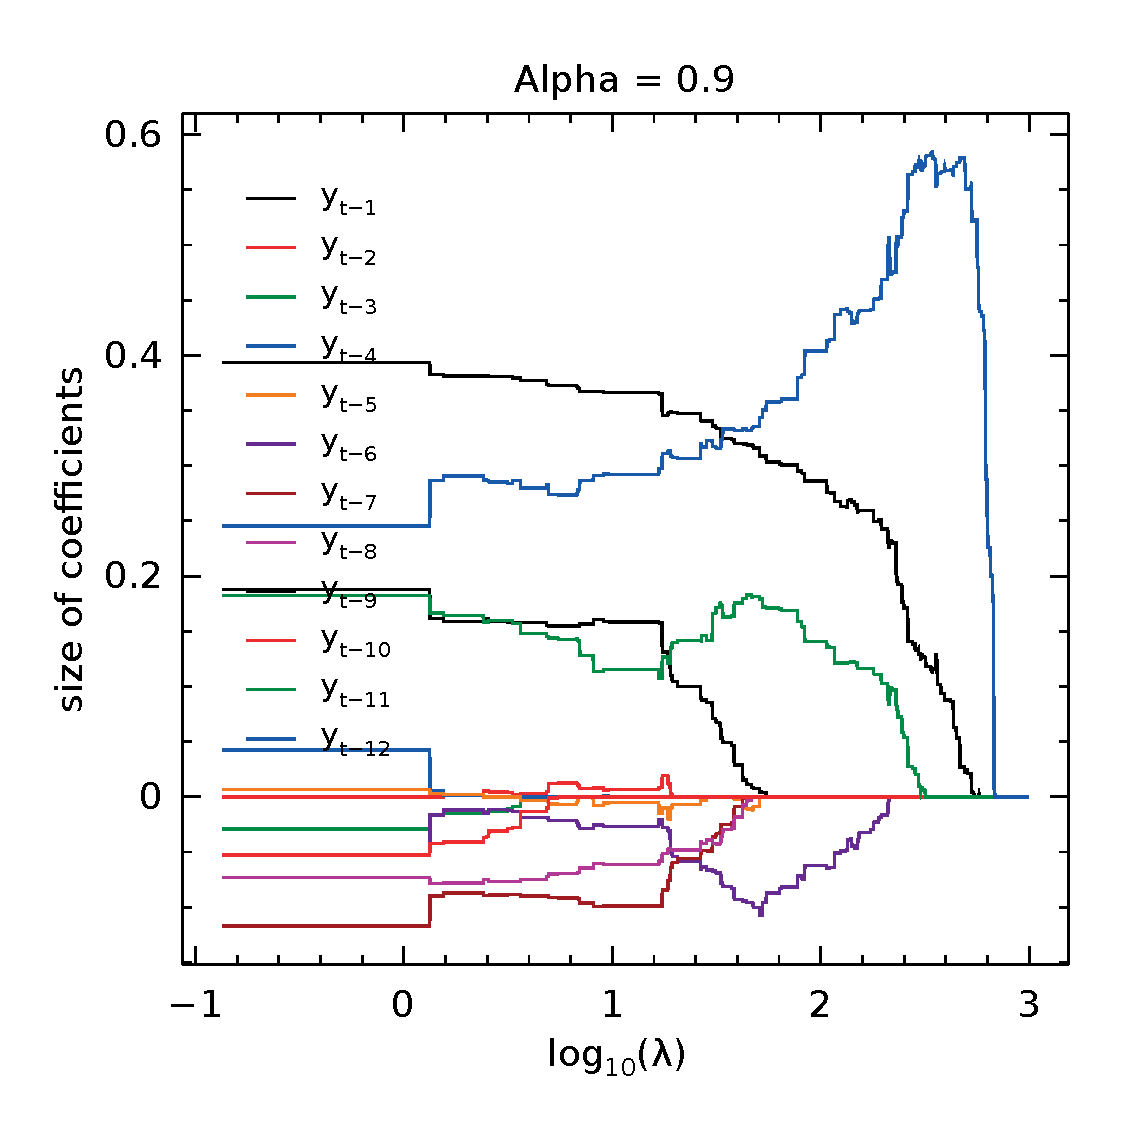
\includegraphics[width=\textwidth]{Figuras/selecao-lasso/par-sellasso-09.pdf}
    \end{minipage}
     \begin{minipage}[b]{\linewidth}
      \centering     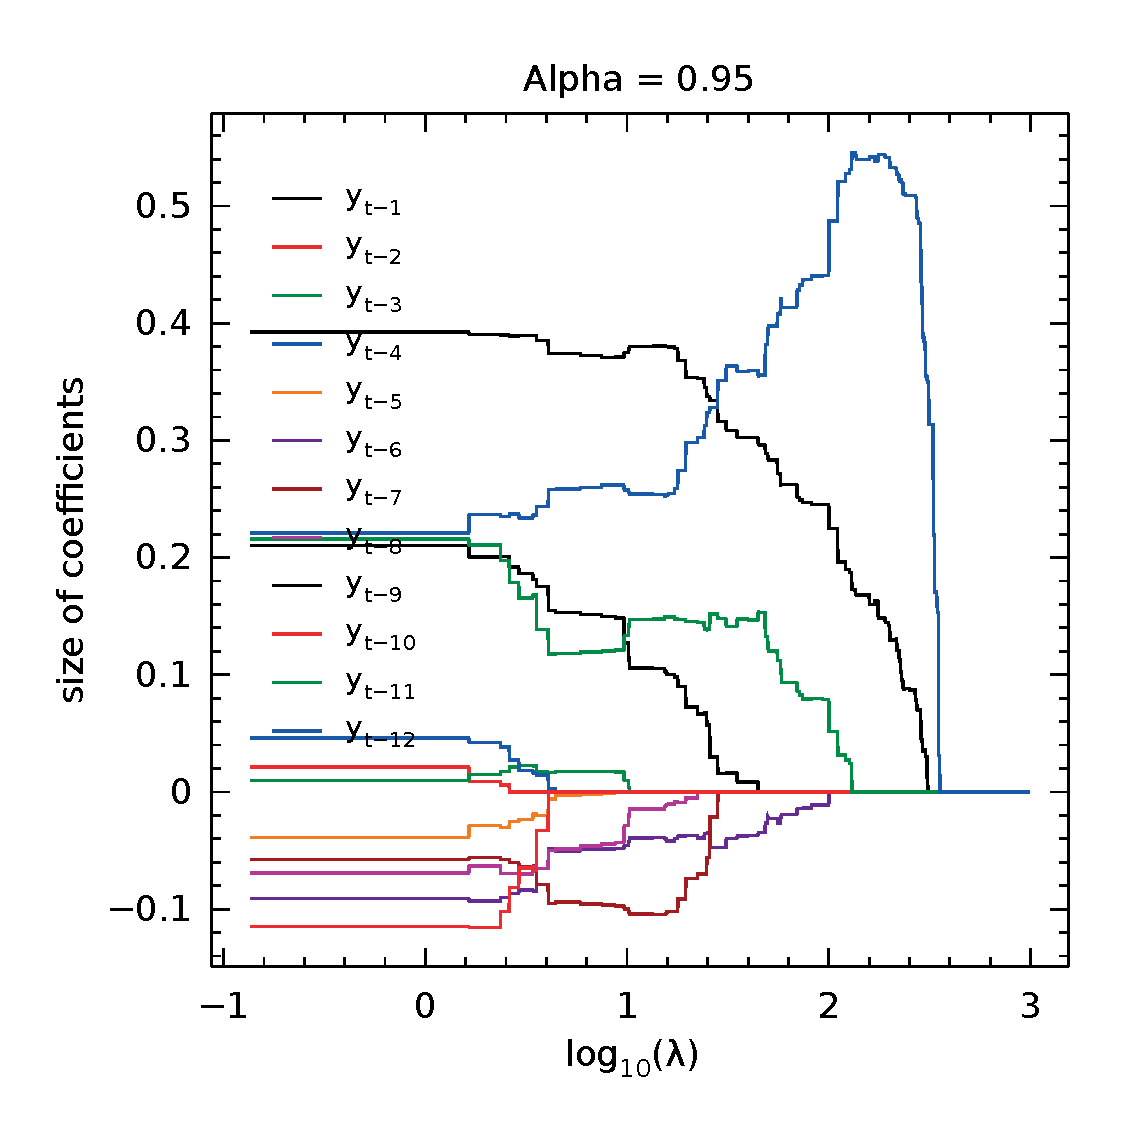
\includegraphics[width=\textwidth]{Figuras/selecao-lasso/par-sellasso-095.pdf}
      \label{fig:npqar-cross}
     \end{minipage}
  \end{minipage}
  \caption{Coefficients path for a few different values of $\alpha$-quantiles. $\lambda$ is presented in a $\log_{10}$ scale, to make visualization easier.}
  \label{fig:npqar-results}
\end{figure}

It is important to mention that even though we have coefficients that are estimated by this method, we don't use them directly. Instead, the nonzero coefficients will be the only covariates used as explanatory variables of a regular quantile autoregression, solved by the linear programming problem \ref{eq:qar-lp}. In summary, the optimization in equation \ref{eq:l1-qar-optim} acts as a variable selection for the subsequent estimation, which is normally called the post-lasso estimation \cite{belloni2009least}.

We are interested, finally, in finding the post-lasso coefficients $\beta_\lambda^*$, which is the solution of the optimization problem given below:
\begin{equation}
\begin{aligned} \beta_\lambda^{*} = \argmin_{\beta_0,\beta,\varepsilon_{t}^{+},\varepsilon_{t}^{-}} & \sum_{t=1}^{n}\left(\alpha\varepsilon_{t}^{+}+(1-\alpha)\varepsilon_{t}^{-}\right)\\
\mbox{s.t. } & \varepsilon_{t}^{+}-\varepsilon_{t}^{-}=y_{t} - \beta_0 - \sum_{p\in L_\lambda} \beta_p x_{t,p},\qquad\forall t\in\{1,\dots,n\},\\
& \varepsilon_t^+,\varepsilon_t^- \geq 0, \qquad \forall t \in \{1,\dots,n\}.
\end{aligned}
\label{eq:post-lasso}
\end{equation}
Note that only a subset of the $P$ covariates will have nonzero values, which are given by the set 
\begin{equation*}
L_\lambda = \{ p \; | \; p \in \{ 1,\dots,P \}, \; |\beta^{*LASSO}_{\lambda,p}| \neq 0  \}.
\end{equation*}
Hence, we have that
$$\beta^{*LASSO}_{\lambda,p} = 0 \iff \beta^{*}_{\lambda,p} = 0.$$


\subsection{Simulation Study}
\label{sec:simulation-ar1}
If we knew an autoregressive process true model
\[
	y_t = \phi_0 + \sum_{p=1}^{P} \phi_p y_{t-p} + \varepsilon_t,
\]
and knew the error distribution, we could estimate the one-step ahead quantile as the sum $\hat{y}_{t+1} + t_{\alpha}$, where $t_\alpha$ is the $\alpha$-quantile for the error distribution. This means that we would be able to use all developments made on conditional mean estimation and simply add an error to estimate quantiles. 

However, that is not the case. When working with quantile estimation for real data we don't know the generating process exactly. Using a quantile regression model provides us a good solution even without making assumptions about the error distribution. 

We propose simulating an AR(1) model
\begin{equation}
	y_t = \phi_0 +  \phi y_{t-1} + \varepsilon_t,\qquad \varepsilon_t \sim N(0, \sigma_\varepsilon^2),	
\label{eq:sim-true-model}
\end{equation}
and test two approaches to predict the one-step ahead quantile. On the first one, we consider known the process true model, given on equation \ref{eq:sim-true-model}. Thus, our task is to estimate values for $\hat{\phi}_0$, $\hat{\phi}$ and $\hat{\sigma}_\epsilon^2$. In order to calculate the one-step ahead $\alpha$-quantile, we need to compute
\begin{equation}
	\hat{q}^{AR}_{t+1|t}(\alpha) = \hat{y}_{t+1|t} + z_\alpha \hat{\sigma}_\varepsilon,
\end{equation}
where $\hat{y}_{t+1|t} = \hat{\phi}_0 + \hat{\phi} y_{t}$ stands for the one-step ahead conditional mean and $z_\alpha = F^{-1}(\alpha)$, where $F$ is the gaussian distribution function.

On the second approach, we fit a quantile regression by solving problem \ref{eq:qar-lp}. The solution of this optimization problem are coefficients $\hat{\beta}_0$ and $\hat{\beta}$. In order to find the one-step ahead $\alpha$-quantile, we use the following expression:
\begin{equation}
		\hat{q}^{QR}_{t+1|t}(\alpha) = \hat{\beta}_0 + \hat{\beta} y_{t}.
\end{equation}
Note that in both approaches we have one intercept term ($z_\alpha \sigma_\varepsilon + {\phi}_0$ and $\beta_0$) and a coefficient for the first lag ($\phi$ and $\beta$). 

We generate data according to equation \ref{eq:sim-true-model}, with different values for $\phi$ (0.25, 0.5, 0.7 and 0.9) and different signal to noise ratios (0.01, 0.05, 0.1, 0.5, 1). We use the signal to noise ratio (RSN) to form the error variance such that $\sigma_e^2 = \dfrac{\phi_0}{1-\phi} \cdot RSN$. This experiment was run with samples of size $n=20000$. The first half was used to fit coefficients and the second half was used as testing set, on which forecasting was done.

Our first goal is then to evaluate the ability of these two approaches to predict the one-step ahead $\alpha$-quantile for a few selected $\alpha$'s. We define the model $m$ forecasting error $\varepsilon_t^m$ as the quantity 
\begin{equation}
\varepsilon_t^m(\alpha) = \hat{q}^m_{t|t-1}(\alpha) - q_t(\alpha) = \hat{q}^m_{t|t-1}(\alpha) - \phi_0 - \phi y_{t-1} - z_\alpha \sigma_\epsilon.
\end{equation}
We use the Root Mean Squared Error (RMSE) to evaluate forecasting performance, which is defined for the model $m$ as follows:
\begin{equation}
RMSE^m = \sqrt{ \frac{1}{n-1} \sum_{i=2}^{n} \left( \varepsilon_t^m(\alpha) \right)^2}
\end{equation}

On section \ref{sec:simulation-tables}, we show a comparison of RMSE for both approaches. To compare them, we compute their RMSE ratio
\begin{equation}
R^{Q/A} = \dfrac{RMSE^{QR}}{RMSE^{AR}}.
\end{equation}
If $R^{Q/A}$ is smaller than 1, it means that the quantile regression approach performed better in terms of RMSE than the conditional mean based on autoregressive models approach.

Once simulations are executed, we notice forecasting errors are similar for both approaches. The exception being when $\phi$ is large (0.9) and the noise is small ($RSN = 0.01$). In those cases, quantile regression performed on average 10\% better than when using the conditional mean approach.
We also provide tables showing differences for the estimated autoregressive and intercept coefficients on section \ref{sec:simulation-tables}.

\subsection{Model selection}

On sections \ref{sec:best-subset-mip} and \ref{sec:best-subset-ell1}, we presented ways of doing regularization. But regularization can be done with different levels of parsimony. For example, we can select a different number $K$ of variables to be included in the best subset selection via MIP or choose different values of $\lambda$ for the $\ell_1$ penalty. Each of these choices leads to a different model, so one needs to know how to select the best one among the options we have. One way of achieving this is by using an information criteria to guide our decision. 

An information criteria summarizes two aspects. One of them refers to how well the model fits the in-sample observations. The other part penalizes the quantity of covariates used in the model. By penalizing how big our model is, we prevent overfitting from happening. So, in order to enter the model, the covariate must supply enough goodness of fit.
In \cite{machado1993robust}, it is presented a variation of the Schwarz criteria for M-estimators that includes quantile regression. The Schwarz Information Criteria (SIC) adapted to the quantile autoregression case is presented below:
\begin{align} 
\begin{split}
SIC(j) = n \log(\hat{\sigma}_{j})+\frac{1}{2}p_{j}\log n,\label{eq:SIC}
\end{split}					
\end{align}
where $\hat{\sigma}_{j}= \frac{1}{n} \sum_{t=1}^{n} \rho_{\alpha}(y_{t}-x^{T}_{t}\hat{\beta}_{n}(\alpha))$, $\rho_\alpha(\cdot)$  is the penalization function and $p_{j}$ the $j$\textsuperscript{th} model's dimension. This procedure leads to a consistent model selection if the model is well specified. 


% % % Métrica

Optimizing a LP problem is many times faster than a similar-sized MIP problem. One of our goals is to test whether a solution of a model with a $\ell_1$-norm can approximate well a solution given by the MIP problem. We propose an experiment that is described as follows. First, we calculate the quantity $k(\lambda)$ of nonzero coefficients, for each given lambda:
\begin{equation}
k_\lambda = \| \beta^*_\lambda \|_0.
\end{equation}
Then, for each number $K$ of total nonzero coefficients (from 1 until 13, where 1 means that only the intercept is included), there will be a penalty $\lambda^*_K$ which minimizes the SIC:
\begin{equation}
\lambda^*_K = \argmin_\lambda \left\lbrace  SIC\left( k_\lambda \right)  | \, k_\lambda = K \right\rbrace.
\end{equation}
Thus, we can compare the SIC of the best lasso fit where exactly $K$ variables are selected with the SIC selected by the MIP problem, also with $K$ variables selected.

To help us view the difference of results between both methods, we define a distance metric $d$ between the subset of coefficients chosen by each one of them. Let 
\begin{equation}
d(\beta^*_{MIP(K)}, \beta^*_{\lambda^*_K}) =  \frac{1}{2K} \sum_{p=1}^P { \left| I(\beta^*_{MIP(K),p}) - I( \beta^*_{\lambda^*_K,p}) \right| }, 
\label{eq:distance}
\end{equation}
where $I$ is an indicator function such that $I(x) = 0$ if $x = 0$ and $I(x)=1$ otherwise. 

Figure \ref{fig:comparison-lm-results} shows the results of these experiments for quantiles $\alpha \in \{0.05, 0.1, 0.5, 0.9, 0.95\}$. The results point us that for small values of $K$ the distance between coefficients is bigger and where we observe the biggest differences between the SIC values. The minimum SIC value for the MIP problem is usually found between 4 and 6 variables in the model.


\begin{figure}
  \centering
  \begin{minipage}[t]{0.4\linewidth}
    \centering
    \begin{minipage}[t]{\linewidth}
      \centering     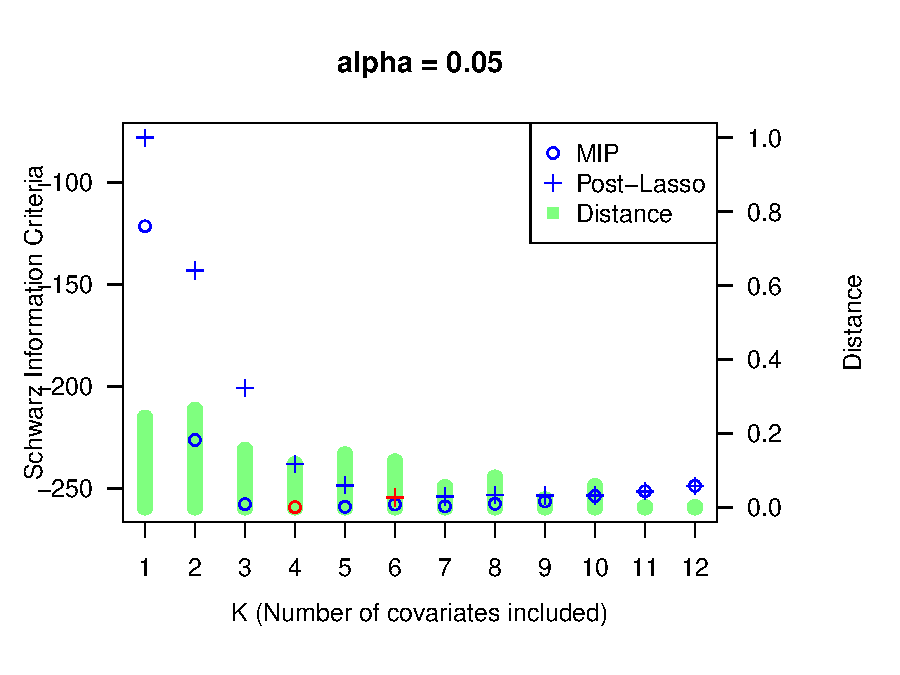
\includegraphics[width=\textwidth]{Figuras/SIC005.pdf}
    \end{minipage}
    \begin{minipage}[b]{\linewidth}
      \centering     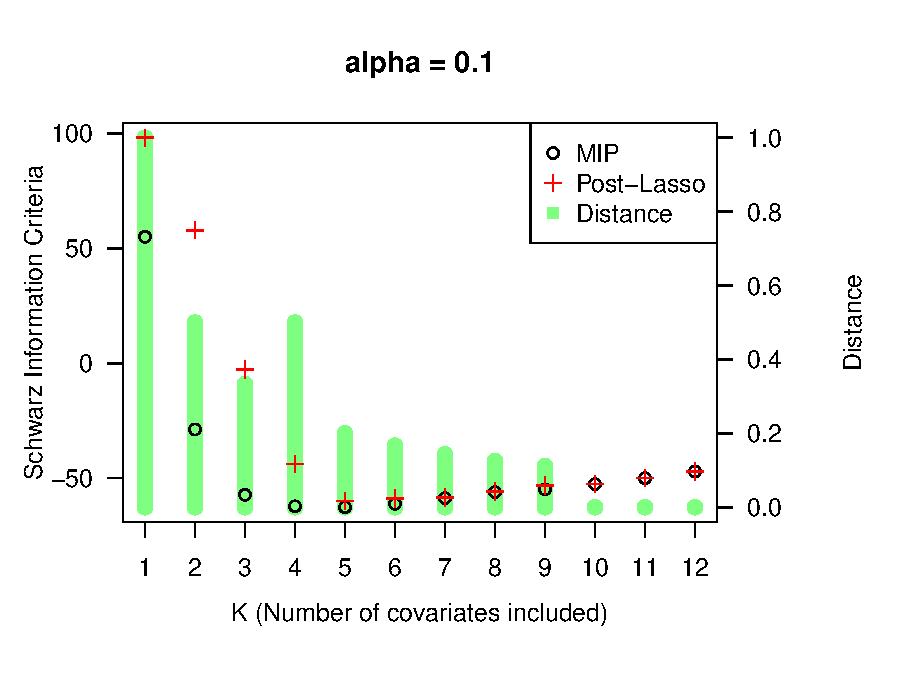
\includegraphics[width=\textwidth]{Figuras/SIC01.pdf}
    \end{minipage}
     \begin{minipage}[b]{\linewidth}
      \centering     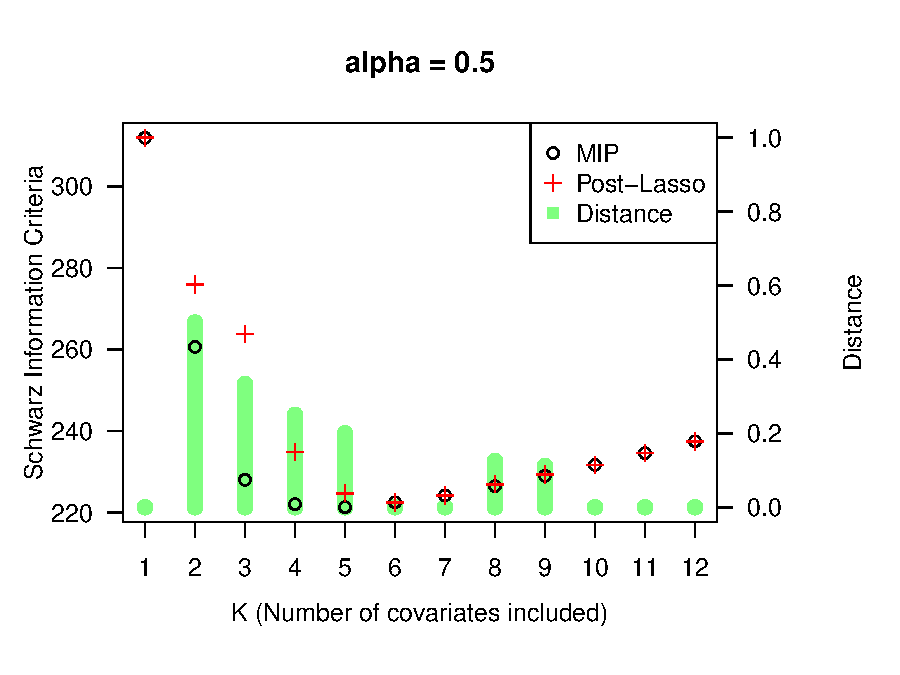
\includegraphics[width=\textwidth]{Figuras/SIC05.pdf}
     \end{minipage}
  \end{minipage}
  \begin{minipage}[t]{0.4\linewidth}
    \centering
    \begin{minipage}[b]{\linewidth}
      \centering     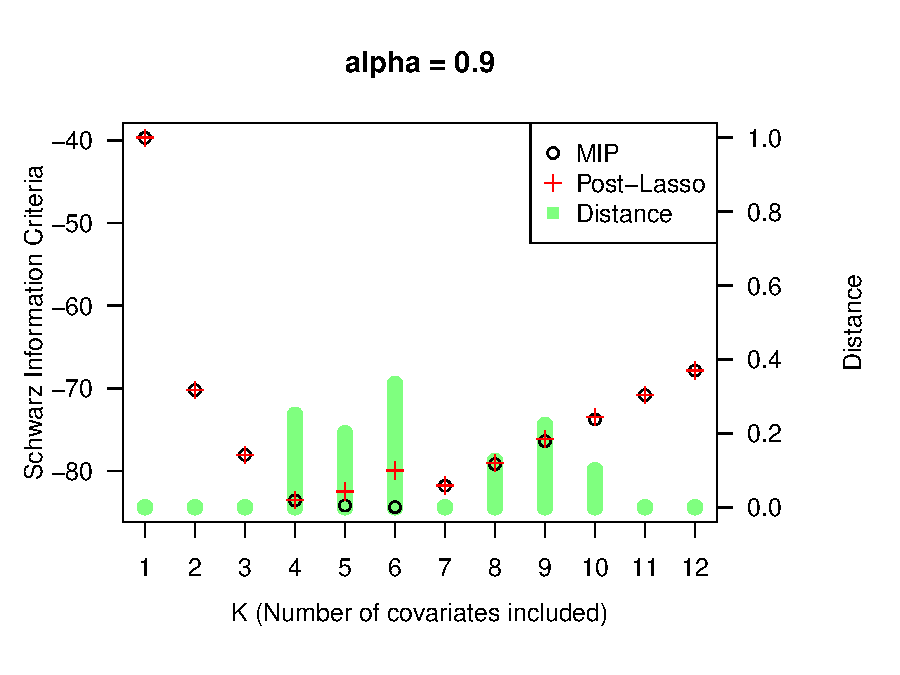
\includegraphics[width=\textwidth]{Figuras/SIC09.pdf}
    \end{minipage}
     \begin{minipage}[b]{\linewidth}
      \centering     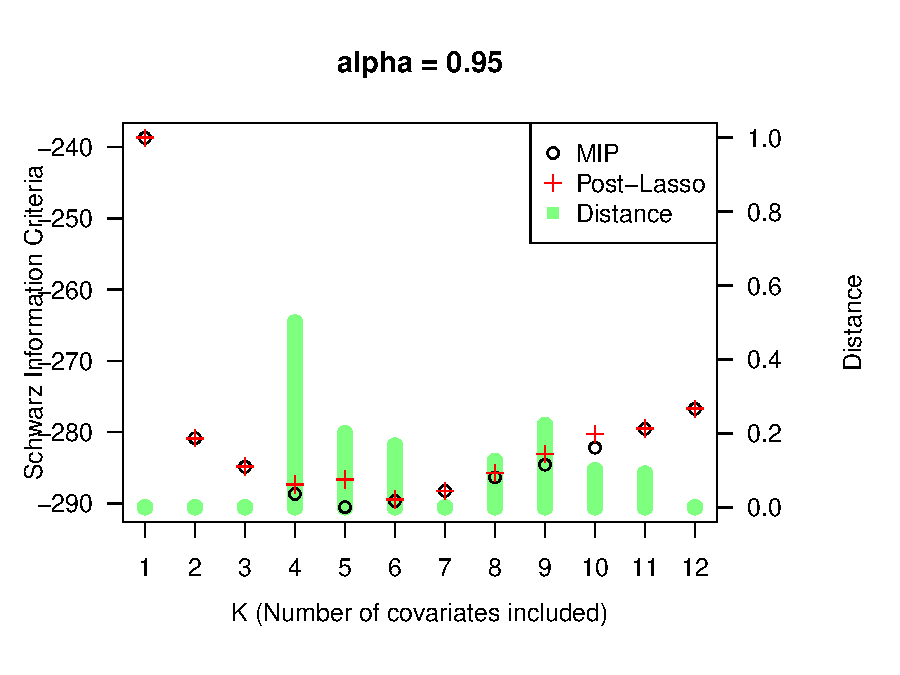
\includegraphics[width=\textwidth]{Figuras/SIC095.pdf}
      \label{fig:npqar-cross}
     \end{minipage}
  \end{minipage}
  \caption{Comparison of SIC between a solution with Lasso as a variable selector and the best subset selection with MIP. The bars represent the distance $d$ as defined by equation \ref{eq:distance}. \\ (*) When the distance is zero, it means that the same variables are selected from both methods for a given $k$. Thus, in these cases we have the same SIC for both of them.}
  \label{fig:comparison-lm-results}
\end{figure}


